%%
% ----------------------------------------------------------------------------
% "THE BEER-WARE LICENSE" (Revision 42):
% <sebastian.rauh@hs-heilbronn.de/michael.bauer@hs-heilbronn.de> wrote this 
% file. As long as you retain this notice you can do whatever you want with 
% this stuff. If we meet some day, and you think this stuff is worth it, you 
% can buy us a beer in return. 
% Michael Lukas Bauer, Sebastian Felix Rauh
% ----------------------------------------------------------------------------
%%

Die in Kapitel 3 aufgeführten Analyse-Ergebnisse wurden für die erste Iteration des Prototyps umgesetzt. Es handelt sich hierbei um einen funktionsfähigen Prototypen, der nativ auf der Apple Watch ausführbar ist. Im folgenden werden Schritte der Umsetzung genauer beschrieben. Hierbei wird auf die Benutzeroberflächenerstellung sowie auf die Verbindung zwischen Uhr und iPhone eingegangen.

\section{Werkzeuge}
Für die Entwicklung wurde Apples Entwicklungsumgebung Xcode in Version 7.2.1 mit den SDKs iOS 9.2 und watchOS 2.1 verwendet. Zum Verwalten des Source-Codes wurde Git\cite{git} eingesetzt. Als Git-Remoteserver wurde Github \cite{github} verwendet. Die graphische Repräsentation der Medikamente sind keine statischen Bilder. Jede Art von Medikament hat eine Vorlage, die dynamisch mit jeglicher Farbe eingefärbt werden kann. Zum Erstellen dieser Vorlagen wurde PaintCode in Version 2.4 \cite{paintCode} genutzt.

\section{Benutzeroberfläche}
\label{ch:userinterface}
Xcode bietet für visuelle Erstellung von Benutzeroberflächen einen eigenen integrierten Editor namens InterfaceBuilder. Hiermit können graphische Elemente per DragAndDrop zu einer Benutzeroberfläche zusammengestellt werden (\ref{fig:xcode-interface-elements}). Ebenfalls per DragAndDrop werden diese Interface-Elemete mit dem Quellcode verbunden (\ref{fig:xcode-interface-code-connect}).

Die Auswahl an Interface-Elementen ist sehr begrenzt und bietet kaum Möglichkeiten eigene Interface-Elemenete zu erstellen. Trotz dieser Begrenztheit lassen sich komplexere Anwendungen bauen.
\begin{figure}
	\caption{Interface Elemente zu Erstellen von Benutzeroberflächen}
	\label{fig:xcode-interface-elements}
	\centering
		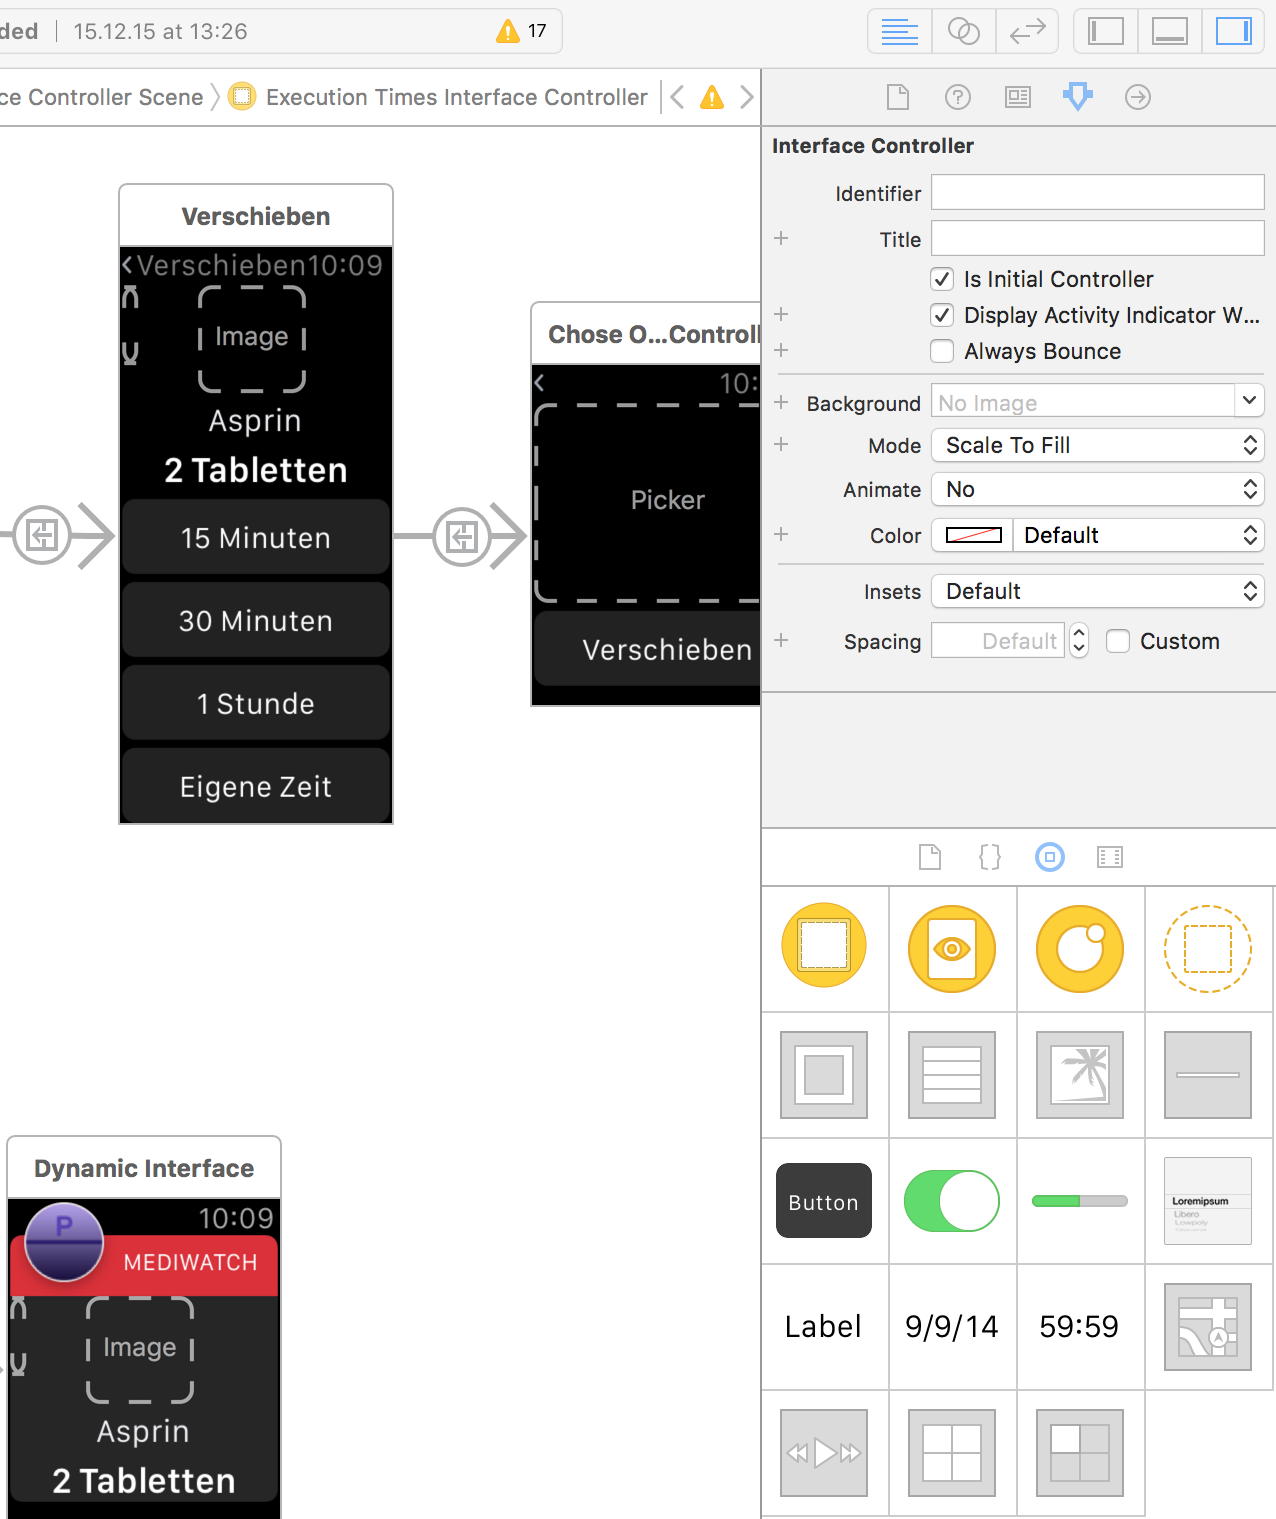
\includegraphics[width=0.9\textwidth]{04_realisation/screenshots/xcode-interface-elements}
\end{figure}

\begin{figure}
	\caption{Interface Elemente mit Quellcode verknüfen}
	\label{fig:xcode-interface-code-connect}
	\centering
	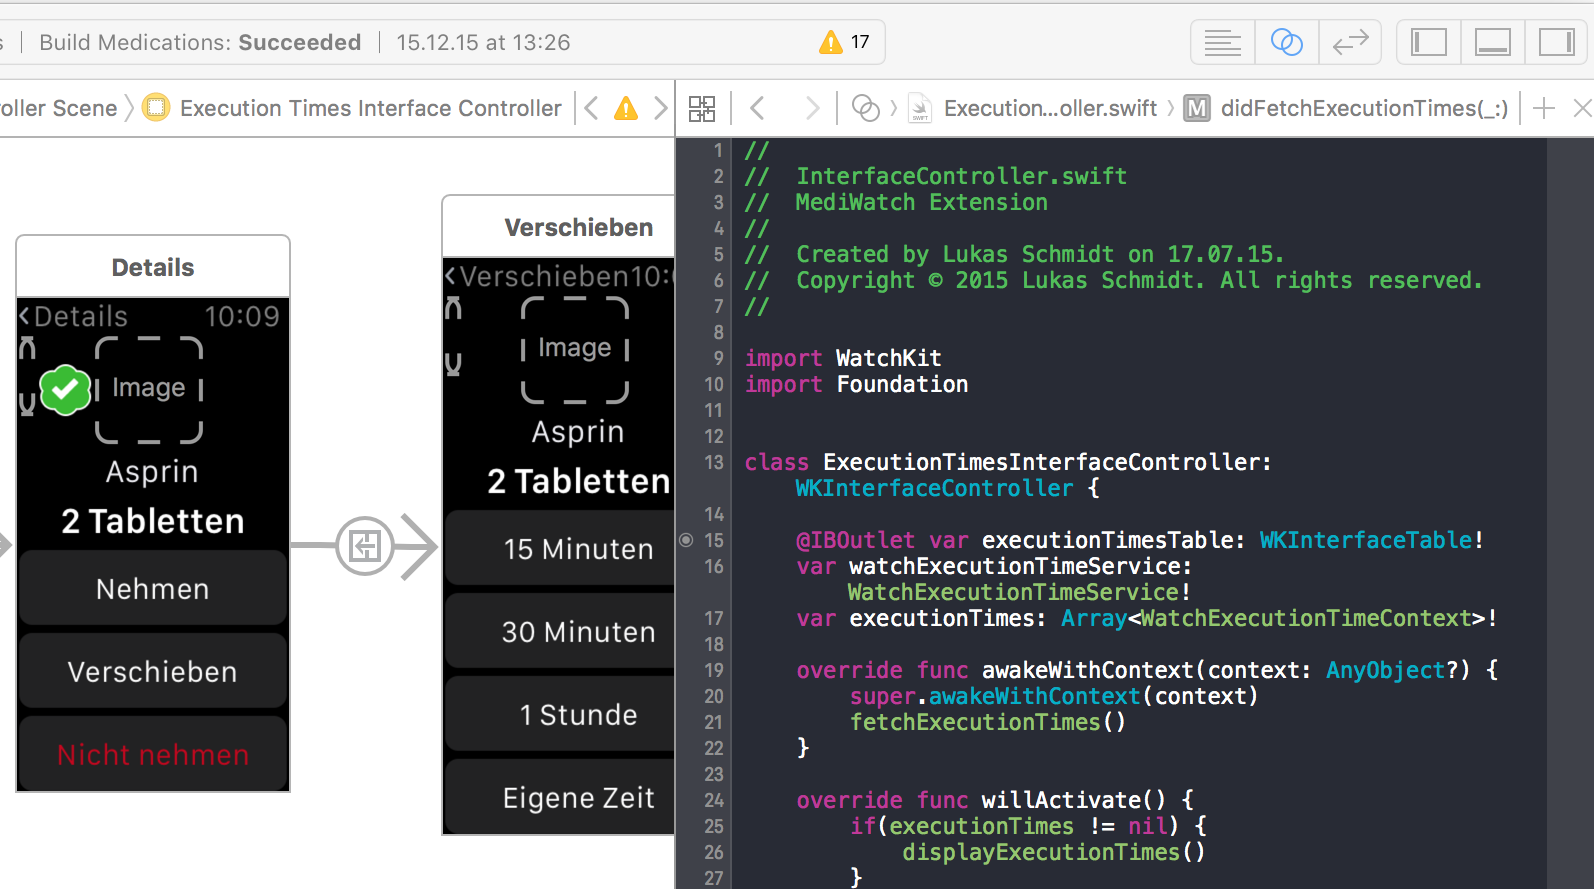
\includegraphics[width=0.9\textwidth]{04_realisation/screenshots/xcode-interface-code-connect}
\end{figure}

\section{Datenhalten - Persistence}
Da generell das iPhone das primäre Objekt der Nutzung ist, bietet sich die Datenhaltung auf dem iPhone an. Apple bietet mit CoreData \cite{Apple:2015swiftOpen} eine Framework zur Persistierung von Objekt-Graphen. Das Framework, welches auf SQLite aufsetzt, bietet eine gute Abstraktion einer Datenbank und ist deswegen leicht und schnell zu integrieren. So bringt CoreData einen graphischen Editor mit, der es erlaubt Datenschemata zu erstellen und diese in Klassen zu transformieren. Daten, die in CoreData gespeichert wurden, lassen sich mittels gezielter Datenbankanfragen abfragen. So muss keine eigene Logik zum Suchen und Sortieren implementiert werden. Des Weiteren bietet CoreData Schnittstellen zur Benachrichtigung bei Änderung in den Daten. Durch langjähriges Bestehen des CoreData Frameworks lässt sich eine stabile Nutzung garantieren. CoreData lässt sich auch auf der AppleWatch nutzen. Dupliziert man nun die Datenhaltung vom iPhone auf die Uhr, müssen diese beiden Datensätze immer konsistent gehalten werden. Dieser Abgleich bei Änderung einer Datenhaltung ist aufwendig zu implementieren. Wird dieser Abgleich jedoch realisiert, ist die Uhr nochmal ein Stück unabhängiger. 

Im konkreten Fall wurde keine doppelte Datenhaltung genutzt. Das iPhone ist also die zentrale Datenquelle. Die Apple Watch kann als Client betrachtet werden, der die Daten des iPhones präsentiert. Zur Realisierung einer Client-Server Verbindung zwischen Uhr und iPhone wurde das WatchConnectivity Framework genutzt, welches in \ref{watchCon} beschrieben wird. Daten müssen vor dem Versenden an die Uhr jedoch immer in ein serialisierbares Format übertragen werden. CoreData Objekte  können nicht direkt übertragen werden.


\section{WatchConnectivity}
\label{watchCon}
Wichtig für die Kommunikation zwischen Uhr und iPhone ist das WatchConnectivity Framework \cite{Apple:2015SharingDataToWatch}. Hierbei ist im Listing \ref{lst:wcConnect} zu sehen, wie genau eine Verbindung aufgebaut werden kann. Es wird auch demonstriert, wie ein Datenaustausch realisiert werden kann. Wichtig ist, dass diese Verbindung zum richtigen Zeitpunkt im Application-Lifecycle aufgebaut wird, da es sonst zu Datenverlusten kommen kann.

\lstinputlisting[caption=Nutzung des WatchConnectivity Framework, label=lst:wcConnect]{04_realisation/code/WatchExecutionTimeService.swift}
 

Mit der \lstinline{sendMessage:} Methode können Nachrichten und Datenpakete gesendet werden, welche sich durch eine ID identifizieren lassen. Eine direkte Antwort auf eine solche Nachricht ist mittels eines Replay-Handlers möglich. So kann eine Art Request/Response Datentransfer realisiert werden. Zu beachten ist jedoch, dass die Kommunikation relativ langsam ist. Sie sollte nur verwendet werden, um kleine Informationen zu senden.

Werden erst beim Watch-App Start benötigte Daten vom iPhone angefordert, kann dies zu einer großen Verzögerung führen. Daher sollten Informationen, die auf der Uhr angezeigt werden, nicht erst zum Zeitpunkt der Darstellung angefordert werden. Gibt es eine Datenänderung auf dem iPhone, die relevante Daten für die Uhr enthält, so sollten diese mit der Methode \lstinline{transferUserInfo:}  an die Uhr gesendet werden. Mit dem Aufrufen dieser Methode wird die übergebene Information nicht direkt zur Uhr geschickt. Das System sendet die Daten zu einem optimalen Zeitpunkt (starke Verbindung zur Uhr, mögliche WLAN Verbindung) an die Uhr. Wenn nun die Watch-App startet, sind die Daten bereit und können direkt dargestellt werden.

Zum Übertragen von größeren Daten steht die Methode \lstinline{transferFile:} zur Verfügung. Die Methode verhält sich equivalent zu \lstinline{transferUserInfo:}, wird jedoch in der Realisierung nicht verwendet.

\section{Modellierung des Programmablaufes}
Apple empfiehlt für iOS und auch watchOS die Nutzung von \gls{mvc} als Grundlage zur Entwicklung von Anwendungen. So existiert in watchOS die Klasse \lstinline{WKInterfaceController} als Supertyp für jeden ViewController. Jeder ViewController ist standardmäßig für einen logischen Bildschirm zuständig. So wird hier als Beispiel in Listing \ref{lst:viewController}  der Controller zur Darstellung von Medikamentendetails beschrieben.

Die mit \lstinline{IBOutlet} annotierten Variablen sind Referenzen für View Elemente. So hält \lstinline{drugNameLabel} ein Label zur Darstellung des Medikamentennamens. Methoden, die mit \lstinline{IBAction} annotiert sind, sind Aktionen, die bei der Interaktion mit dem Interface vom Nutzer ausgelöst werden. \lstinline{onTakeMedication} wird ausgelöst, wenn der Nutzer den Button zur Bestätigung der Einnahme klickt. Der Prefix \lstinline{IB} steht bei den Annotationen für InterfaceBuilder, welcher zum Erstellen der View-Elemente genutzt wird (\ref{ch:userinterface}).

Zum Wechseln zwischen ViewControllern, also z.B. von der Darstellung einer Liste zu einer Detailansicht, führt Apple den Begriff Segue ein. Ein Segue beschreibt einen Übergang zwischen zwei ViewControllern. Es gibt zwei Typen von Segues: Push und Modal. Ein modaler Segue fährt vom unteren Rand des Bildschirms über den vorherigen ViewController. Diese Interaktion fordert den Nutzer auf, eine Eingabe oder Interaktion zu tätigen. Ist diese Interaktion erfolgt, verschwindet der ViewController wieder nach unten. Der Push Segue eignet sich für mehrdimensionale Interaktionen. Eine ideale Anwendung dafür ist, Informationen im Detail anzuzeigen. Der Segue verdeckt von der rechten Seite  den aktuellen ViewController. Diese Interaktion vermittelt dem Nutzer eine Kontinuität. So kann dieser Segue sehr gut hintereinander genutzt werden, um immer tiefer in eine Informationsstruktur vorzudringen. Der Segue lässt sich durch einen Button am oberen linken Rand wieder verlassen. Auch eine Wischgeste, die dem Nutzer erlaubt den ViewController wegzuschieben, ist vorhanden. Der Push Segue ist den meisten Nutzern auch von iOS bekannt.

Durch die geringe Anzahl an Segues kann eine sehr konsistente Interaktion auf der ganzen Plattform garantiert werden. Dies erleichtert dem Nutzer die Navigation.

Die überschriebene Methode \lstinline{awakeWithContext:} ist eine Lifecycle Methode des ViewControllers. Sie wird immer nach dem Erstellen des ViewControllers ausgeführt. Sie hilft, Daten von einem ViewController zum nächsten zu geben. Die Daten werden vom vorhergehenden ViewController bereit gestellt. Dieser überschreibt \lstinline{contextForSegue WithIdentifier:} und kann nun Daten abhängig vom Identifier übergeben. So sind diese zwei Methoden der einzige Kontaktpunkt von ViewControllern. Dies erhöht extrem die Kapselung der Komponenten.

\lstinputlisting[caption=ViewController zur Darstellung von Medikamentendetails, label=lst:viewController]{04_realisation/code/MedicationDetailsController.swift}

\section{Picker - Auswahl}
Mit \lstinline{WKInterfacePicker} bietet Apple eine Standard View-Componente zum Auswählen von Elementen aus einer Liste. Der Nutzer kann so mit der Digital-Crown die Elemente selektieren. Diese leicht zu integrierende View-Komponente ist einfach zu bedienen und hebt das Nutzungserlebnis von anderen Uhren ab. Mit dieser Komponente wird die Auswahl realisiert, mit der der Nutzer die Zeit zum Verschieben des Medikamentes wählt.

\section{Notification Management}
Notifications für die Medikationen werden mit der Notification API  registriert \cite{Apple:2015notif}. Auch kann das Verhalten der Notifications angepasst werden. So können vordefinierte Aktionen wie \glqq Einnehmen\grqq  oder \glqq Verschieben\grqq in die Notifications konfiguriert werden.

Bei der Notification handelt es sich um eine UILocalNotification \cite{Apple:2015notif}. Die Art von Notification benötigt keinen \gls{remoteServer}, sondern wird vom verbundenen iPhone verwaltet. Zum jetzigen Zeitpunkt ist es nicht möglich UILocalNotification von der Uhr zu erstellen. Dies würde die Uhr im Falle der Mediwatch-Anwendung noch unabhängiger machen. Sind die Notifications einmal auf dem iPhone registriert, werden sie zum Ausführungszeitpunkt auf der Uhr angezeigt. Dazu ist keine Verbindung zum iPhone mehr nötig.

\section{Anwendung}

Die Anwendung besteht aus zwei Komponenten auf der Apple Watch. Eine native Notification  und eine auf der Uhr installierte und ausgeführte Anwendung (siehe \ref{ch:watch_software}). In \ref{fig:watch-real} finden sich Bilder der Anwendung auf der Uhr. Dies sind Screenshots, die mit Hilfe einer Bildbearbeitungssoftware eingefügt wurden. Diese Bilder können ein Gefühl für die echte Anwendung auf der Uhr vermitteln.

\subsection{Notification}
 Die Notification bringt die Uhr zum Zeitpunkt der geplanten Medikamenteneinnahme zum Vibrieren und lässt optional einen Ton erklingen. Dies führt dazu, dass der Anwender auf die Uhr blickt und an die bevorstehende Medikamenteneinnahme erinnert wird. Die Notification wurde daraufhin optimiert, sodass eine große graphische Repräsentation des Medikaments angezeigt wird. Dem Nutzer wird so die Wiedererkennung des Medikaments erleichtert (siehe \ref{fig:watch-app-notification}). Neben dem Medikamentennamen wird auch die Dosierung des Medikaments dargestellt. Mit nur einer Aktion wird dem Nutzer ermöglicht, die Medikamenteneinnahme zu bestätigen oder sie zu verschieben. Die Notification ist darauf ausgelegt eine sehr schnelle Interaktion zu ermöglichen, damit der Nutzer nicht länger als 10 Sekunden mit der Uhr interagieren muss (siehe \ref{fig:watch-app-notification}). Diese Zeit führt sich auf die Studie \glqq Smartwatch in vivo\glqq \cite{Pizza:2016} zurück.
 
 Diese Erweiterung der Notification mit dem Bild des Medikaments wird jedoch vom System geregelt. Dauert das Rendern der Notification zu lange, stellt das System eine reine Textdarstellung der Notification dar. Dies führt zu einem gewaltigen Informationsverlust. Als Anwendungsentwickler hat man nur die Option, seine Notification mit bestmöglicher Geschwindigkeit zu rendern, um eine Textdarstellung zu vermeiden. Das System bietet jedoch keine Garantie für eine erweiterte Darstellung der Notification. Dies kann im Extremfall zu Verwirrungen des Nutzers führen.
\begin{figure}
	\caption{Notification für ein Medikament}
	\label{fig:watch-app-notification}
	\centering
	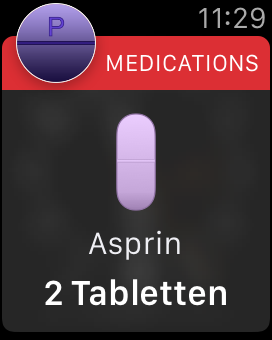
\includegraphics[width=0.4\textwidth]{04_realisation/screenshots/watch/notification01.png}
	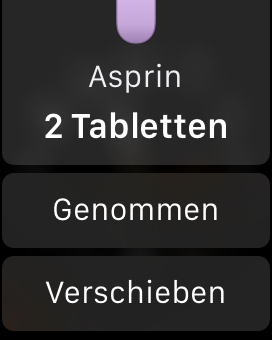
\includegraphics[width=0.4\textwidth]{04_realisation/screenshots/watch/notification02.png}
\end{figure}

\subsection{Native Anwendung}
Neben der Notification gibt es noch eine native App. Diese läuft auf der Uhr und stellt eine Liste der Medikamente des aktuellen Tages dar. Die App muss aktiv vom Nutzer gestartet werden. Der Nutzer muss also auf die Digital Crown drücken und dann die App aus der Übersicht wählen. In Abbildung \ref{fig:watch-app-take} wird ein Medikament aus der Liste ausgewählt. Nachdem man ein Medikament ausgewählt hat, bekommt man in einer Detailansicht das Medikament zu sehen. Nun kann das Medikament als genommen oder nicht genommen markiert werden. Ein visuelles Feedback (grüner Haken) zur Einnahme zeigt dem Nutzer seine Aktionen an. Von der Detailansicht aus ist es auch möglich, ein Medikament zur späteren Einnahme zu markieren. Hier hat der Anwender die Möglichkeit aus vordefinierten Zeiten auszuwählen oder eine eigene Zeit zu bestimmen. Um die gewählte Zeitdauer wird die Benachrichtigung für das Medikament verschoben (siehe \ref{fig:watch-app-delay}). 

\begin{figure}
	\caption{Native Anwendung: Interface zum Wählen eines Medikaments (oben links). Medikament als genommen bestätigen (oben rechts). Eigene Zeitdauer auswählen (unten links). Medikament ist in der Übersicht als verschoben markiert (unten rechts)}
	\label{fig:watch-app-take}
	\centering
	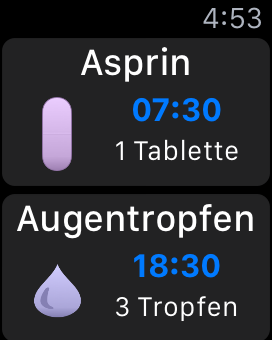
\includegraphics[width=0.4\textwidth]{04_realisation/screenshots/watch/notTaken01.png}
	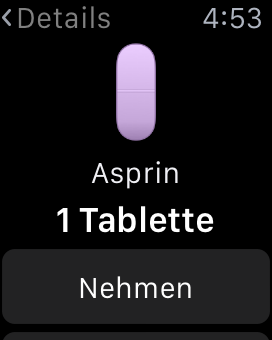
\includegraphics[width=0.4\textwidth]{04_realisation/screenshots/watch/notTaken02.png}
	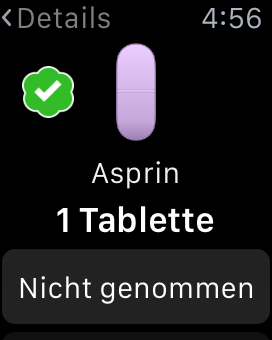
\includegraphics[width=0.4\textwidth]{04_realisation/screenshots/watch/taken01.png}
	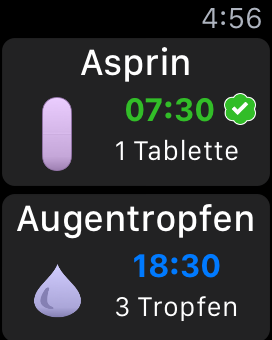
\includegraphics[width=0.4\textwidth]{04_realisation/screenshots/watch/taken02.png}
\end{figure}

\begin{figure}
	\caption{Native Anwendung: Interface zum Verschieben eines Medikaments (oben links). Zeitdauer für das Verschieben wählen (oben rechts). Medikament ist als genommen markiert (unten links). Medikament ist in der Übersicht als genommen markiert(unten rechts)}
	\label{fig:watch-app-delay}
	\centering
	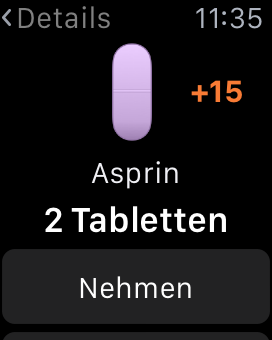
\includegraphics[width=0.4\textwidth]{04_realisation/screenshots/watch/delay01.png}
	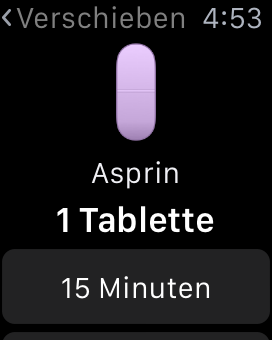
\includegraphics[width=0.4\textwidth]{04_realisation/screenshots/watch/delay02.png}
	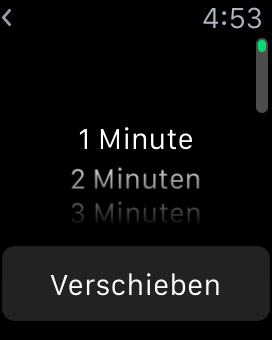
\includegraphics[width=0.4\textwidth]{04_realisation/screenshots/watch/delay03.png}
	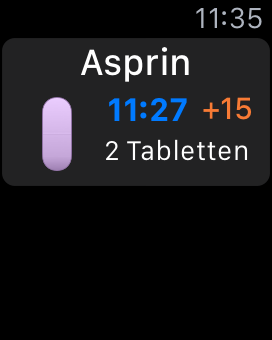
\includegraphics[width=0.4\textwidth]{04_realisation/screenshots/watch/delay04.png}
\end{figure}


\begin{figure}
	\caption{Native Anwendung - dargestellt auf realen Apple Watches}
	\label{fig:watch-real}
	\centering
	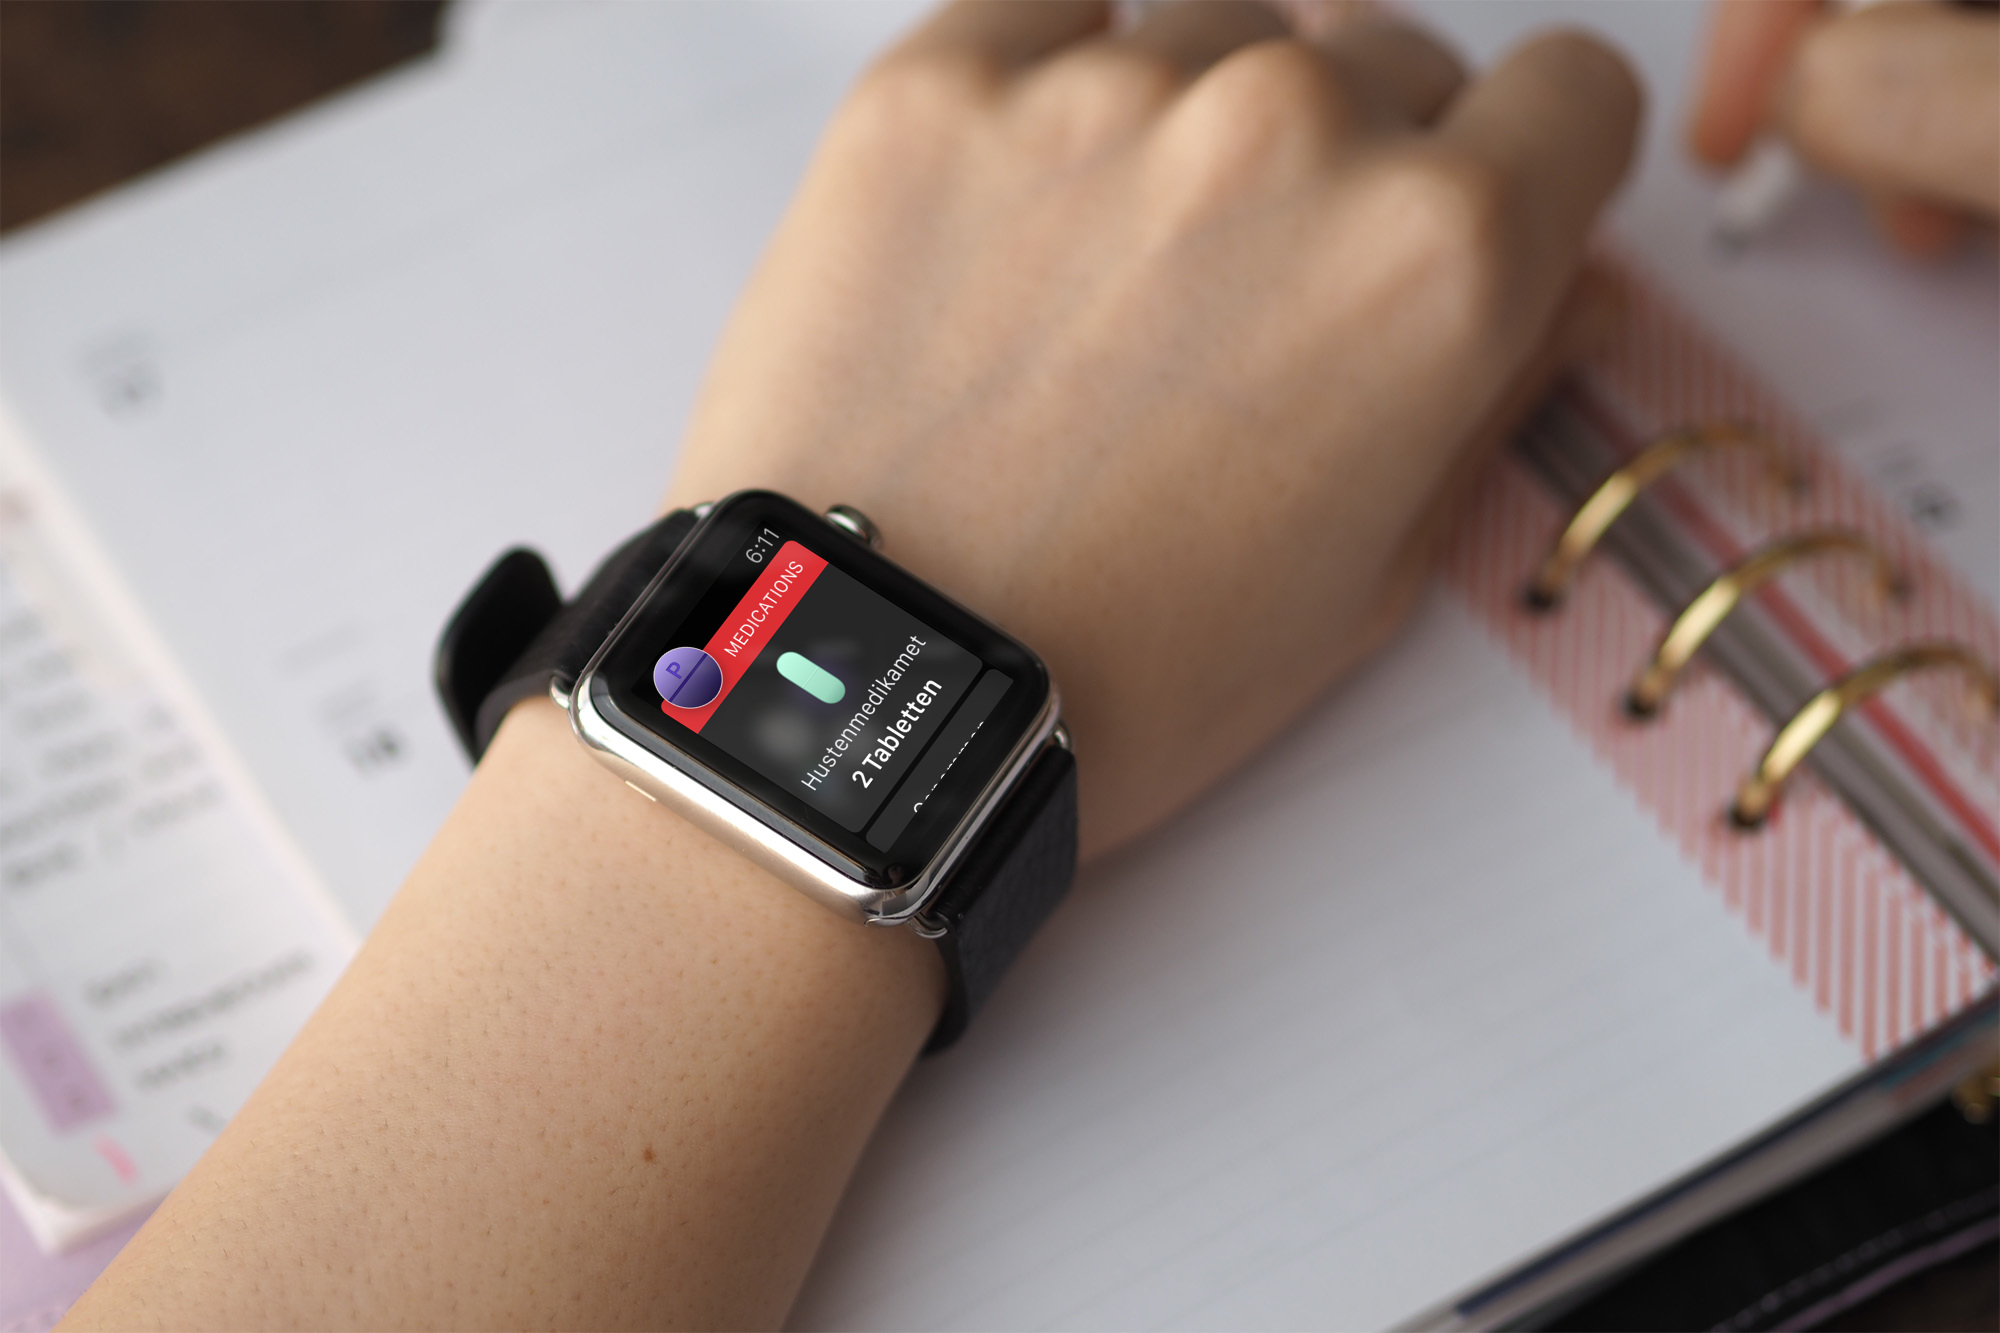
\includegraphics[width=1\textwidth]{04_realisation/screenshots/Mockup-Generated-by-Dunnnk.jpg}
	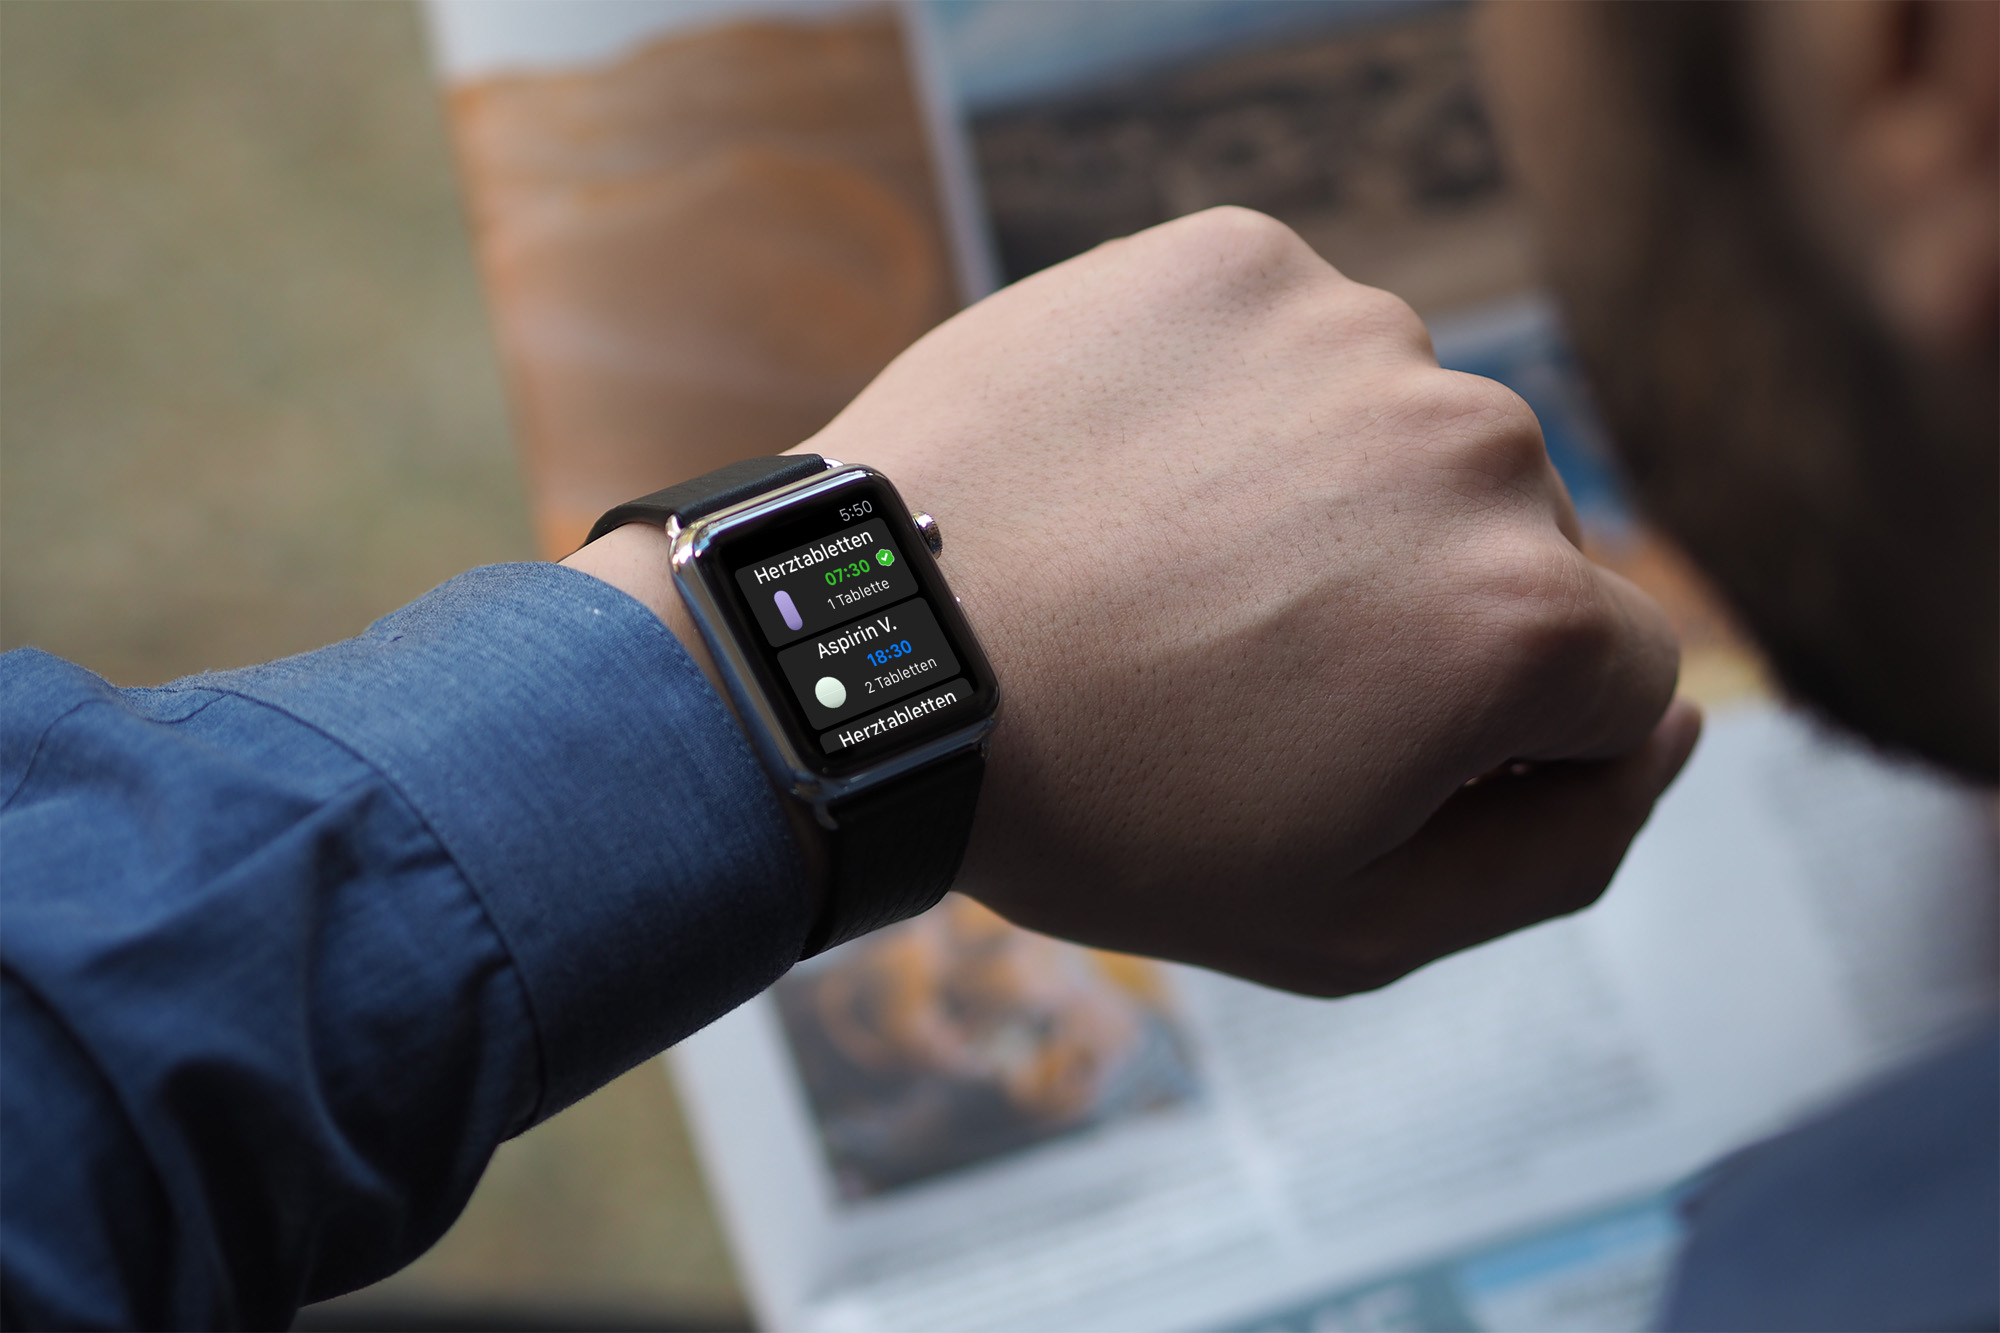
\includegraphics[width=1\textwidth]{04_realisation/screenshots/Mockup-Generated-by-Dunnnk-2.jpg}
	\end{figure}
\section{Quellcode}
Das ausführbare Projekt lässt sich von Github unter folgender URL\cite{Schmidt:repoCode} auschecken. So kann es kompiliert und getestet werden. 

